%% LyX 2.3.6.1 created this file.  For more info, see http://www.lyx.org/.
%% Do not edit unless you really know what you are doing.
\documentclass[english]{article}
\usepackage[T1]{fontenc}
\usepackage[latin9]{inputenc}
\usepackage{geometry}
\geometry{verbose,tmargin=2.5cm,bmargin=2.5cm,lmargin=2.5cm,rmargin=2.5cm}
\usepackage{calc}
\usepackage{graphicx}
\PassOptionsToPackage{normalem}{ulem}
\usepackage{ulem}

\makeatletter

%%%%%%%%%%%%%%%%%%%%%%%%%%%%%% LyX specific LaTeX commands.
%% Because html converters don't know tabularnewline
\providecommand{\tabularnewline}{\\}

\makeatother

\usepackage{babel}
\begin{document}

\section{9597 ALVL 2017}

\subsection{Paper 1}
\begin{enumerate}
\item \textbf{{[}DHS/PRELIM/9597/2017/P1/Q1{]} }

The variable length record file \texttt{SEAGAMES2007\_2015.csv} contains
the results of SEA Games from 2007 to 2015.

\subsection*{Task 1.1 }

Determine the country with the most number of medals and the corresponding
medal count during this period.

Sample output:

\texttt{Most number of medals (999): CountryX}

\subsection*{Evidence 1 }

Program code.\hfill{} {[}6{]}

\subsection*{Evidence 2}

Screenshot.\hfill{} {[}1{]}

\subsection*{Task 1.2 }

Determine the year(s) in which the host country also topped the medal
rally (i.e. won the most number of gold medals).

Sample output: 

\texttt{CountryY (999 Gold medals): YearZ}

\subsection*{Evidence 3}

Program code. \hfill{}{[}7{]}

\subsection*{Evidence 4}

Screenshot.\hfill{} {[}1{]}

{[}SPLIT\_HERE{]}
\item \textbf{{[}DHS/PRELIM/9597/2017/P1/Q2{]} }

The following shows an incomplete recursive linear search algorithm.

\noindent %
\noindent\begin{minipage}[t]{1\columnwidth}%
\texttt{LinearSearch(data, target, first): }

\texttt{if \# base case 1 (not found)}

\texttt{\qquad{}return -1 }

\texttt{if target == data{[}0{]}: \# base case 2 (found) }

\texttt{\qquad{}return first}

\texttt{\# recursive case }

\texttt{return LinearSearch(data{[}1:{]}, target, ?)}%
\end{minipage}

The third parameter \texttt{first} keeps track of the original index
of the first item in the list \texttt{data}.

\subsection*{Task 2.1}

Write program code to implement the above recursive search algorithm.
Test your implementation with appropriate test data. 

\subsection*{Evidence 5}

Program code. \hfill{}{[}5{]}

\subsection*{Evidence 6 }

Screenshot. \hfill{}{[}2{]}

\subsection*{Task 2.2}

Make slight modifications to make your recursive linear search more
efficient. You should provide appropriate comments to explain how
and why your improved recursive linear search is more efficient. 

\subsection*{Evidence 7}

Program code. \hfill{}{[}6{]}

\subsection*{Evidence 8}

Screenshots. \hfill{}{[}2{]}

{[}SPLIT\_HERE{]}
\item \textbf{{[}DHS/PRELIM/9597/2017/P1/Q3{]} }

In line with Singapore's Smart Nation vision, Dunman Pre-School library
decides to go digital to convert their physical books collection to
e-books. You have been tasked to organise book and borrower information
using your knowledge and skills in OOP and data structures. 

The library will maintain the books information using a binary search
tree (BST). Each BST node contains BookID, Title, OnLoan (the number
of copies currently on loan). For copyright reason, the library will
make available 3 digital copies of each title for loan. Each BST node
will thus contain an array of borrower's details: BorrowerID, BorrowDate,
ReturnDate. The default loan period is 10 days. Books which are overdue
incur a fine of \$0.15 per day. 

When a book is loaned, an entry is made in an available array position.
When it is Returned, the BorrowerID value will be set to -1. Items
which are returned will also have the information appended to a serial
fixed length record file TRANSACTION.txt with the following structure
(Dates are stored in YYYYMMDD format): 
\noindent \begin{center}
\texttt{<ReturnDate><BorrowerID><BookID><BorrowDate> }
\par\end{center}

\subsection*{Task 3.1 }

Using OOP techniques, setup the BST structure and perform insertion
of books information from \texttt{BOOKS.txt.} You should take the
necessary preprocessing step to ensure optimal search performance. 

\subsection*{Evidence 9}

Program code. \hfill{} {[}8{]}

\subsection*{Task 3.2}

Write additional program code to update the BST with loan information
from \texttt{LOAN.txt} which has the following structure: 
\noindent \begin{center}
\texttt{<Action><BorrowerID><BookID><BorrowDate/ReturnDate> }
\par\end{center}

where Action has two possible options: \texttt{B} (borrow) and \texttt{R}
(return), as well as search capabilities for book and borrower. 

\subsection*{Evidence 10}

Program code. \hfill{}{[}10{]}

\subsection*{Evidence 11}

Screenshot for output on query for BookIDs \texttt{978-0-9746475-0-0}
and \texttt{978-1-942824- 04-4}. \hfill{} {[}2{]}

\subsection*{Evidence 12 }

Screenshot for output on query for BorrowerIDs \texttt{T1276249B}
and \texttt{T1395320H}. \hfill{}{[}2{]}

\subsection*{Task 3.3}

Write program code to generate a daily report of borrowers who have
overdue books and output this information to the text file \texttt{OVERDUE.txt}
with the following structure: 

\noindent %
\noindent\begin{minipage}[t]{1\columnwidth}%
\texttt{<CurrentDate> }

\texttt{<BorrowerID><LoanDate><ReturnDate><BookID> }

\texttt{<FineDue> }%
\end{minipage}

The information should be ordered by BorrowerID, followed by descending
order of days overdue, and lastly by BookID. Take CurrentDate to be
20170602.

\subsection*{Evidence 13}

Program code. \hfill{}{[}8{]}

\subsection*{Evidence 14 }

Screenshot of \texttt{OVERDUE.txt}. \hfill{} {[}1{]}

\subsection*{Task 3.4}

To make the program more robust, write validation code for \texttt{BorrowerID}
which is a user's NRIC. For NRIC number in the format SABCDEFG, where
A is the first digit, B is the second digit and so on. 
\begin{enumerate}
\item[1.]  sum = (2{*}A) + (7{*}B) + (6{*}C) + (5{*}D) + (4{*}E) + (3{*}F)
+ (2{*}G) 
\item[2.]  Add 4 to sum if your IC number starts with T or G.
\item[3.]  Find the remainder when sum is divided by 11. 
\end{enumerate}
Convert the remainder into a letter using the following table. Remainder
0 1 2 3 4 5 6 7 8 9 10 Letter (NRIC) J Z I H G F E D C B A Letter
(FIN) X W U T R Q P N M L K 

\subsection*{Evidence 15 }

Program code.\hfill{} {[}6{]}

\subsection*{Evidence 16 }

Screenshot of output for NRICs \texttt{T1276249B} and \texttt{G2873148M}.
\hfill{}{[}2{]}

\subsection*{Task 3.5}

Write program code to determine the top 3 borrowers' IDs and top 3
most popular book titles with cumulative number of loans. 

\subsection*{Evidence 17 }

Program code. \hfill{}{[}7{]}

\subsection*{Evidence 18 }

Screenshot.\hfill{} {[}2{]}

{[}SPLIT\_HERE{]}
\item \textbf{{[}DHS/PRELIM/9597/2017/P1/Q4{]} }

You have been tasked to develop a machine learning algorithm for text
analysis. You have been provided with the following training data
(in CORPUS.txt): 

\noindent %
\noindent\begin{minipage}[t]{1\columnwidth}%
\texttt{I love Computing. Computing rocks, rocks, rocks!}

\texttt{I have a dog and a cat.}

\texttt{Best of Computing? Projects, projects, projects! }

\texttt{My cat keeps chasing my dog. Cats!}%
\end{minipage}

\subsection*{Task 4.1 }

Create and output a frequency dictionary of case-insensitive key terms
for the corpus. For the above data, after removing stop words (eg
I, have, etc.) the key terms will be 
\noindent \begin{center}
\texttt{best, cat, cats, chasing, computing, dog, love, projects,
rocks}
\par\end{center}

\subsection*{Evidence 19}

Program code.\hfill{} {[}5{]} 

\subsection*{Evidence 20}

Screenshot of dictionary contents. \hfill{}{[}1{]}

\subsection*{Task 4.2 }

Create a 2D array to store the frequency of sorted key terms in each
sentence. For example, for the first sentence, the array contents
will be: 
\noindent \begin{center}
\texttt{{[}0, 0, 0, 0, 2, 0, 1, 0, 3{]}}
\par\end{center}

\subsection*{Evidence 21 }

Program code. \hfill{}{[}4{]}

\subsection*{Evidence 22}

Screenshot. \hfill{}{[}2{]}

\subsection*{Task 4.3}

Update your 2D array to give a normalised frequency of each key term
i.e. divide the number of occurrences of each key term in a sentence
by the total number of key terms in the sentence. This gives a more
accurate representation of the importance of the key terms relative
to the length of the sentence. For the first sentence, the updated
weighted array contents will be:
\noindent \begin{center}
\texttt{{[}0, 0, 0, 0, 0.333, 0, 0.167, 0, 0.5{]}}
\par\end{center}

Output your normalised array. 

\subsection*{Evidence 23 }

Program code.\hfill{} {[}5{]}

\subsection*{Evidence 24}

Screenshot.\hfill{} {[}2{]}

\subsection*{Task 4.4 }

Use your normalised array and an appropriate algorithm, divide the
key terms into 2 groups. Output the contents of the 2 groups. 

\subsection*{Evidence 25}

Program code. \hfill{}{[}9{]}

\subsection*{Evidence 26 }

Screenshot.\hfill{} {[}2{]}

{[}SPLIT\_HERE{]}
\item \textbf{{[}DHS/PRELIM/9597/2017/P2/Q1{]} }

Singapore has declared war against diabetes. Health Promotion Board
has devised an online Diabetes Risk Assessment (DRA) tool to help
users assess if they are at risk of developing Type 2 diabetes. 

Fighting against diabetes requires a long-term multi-pronged approach.
You have been engaged as a project manager by Unbelievable Company
to assemble a project team to help devise preventive programmes for
their employees. You have come up with the following PERT chart based
on their DRA results for those employees at risk.
\begin{center}
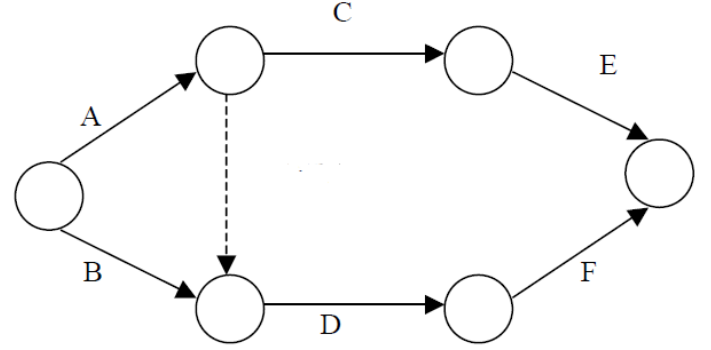
\includegraphics[width=0.5\paperwidth]{C:/Users/Admin/Desktop/Github/question_bank/LyX/static/img/9597-DHS-2017-P2-Q1-1}
\par\end{center}

\noindent \begin{center}
\begin{tabular}{|c|c|c|}
\hline 
Acitivity & Description & Duration(weeks)\tabularnewline
\hline 
A &  & 2\tabularnewline
\hline 
B &  & 3\tabularnewline
\hline 
C &  & 12\tabularnewline
\hline 
D &  & 12\tabularnewline
\hline 
E &  & 2\tabularnewline
\hline 
F &  & 2\tabularnewline
\hline 
\end{tabular}
\par\end{center}
\begin{enumerate}
\item Provide the most appropriate labels (A-F) for the following proposed
activities: 
\begin{itemize}
\item Awareness talk 
\item Exercise regime 
\item Healthy cooking workshop 
\item Healthy eating regime 
\item Pre-Medical examination 
\item Post-Medical examination
\end{itemize}
\item {}
\begin{enumerate}
\item State the critical path and the minimum project completion time.\hfill{}
{[}2{]}
\item Explain the significance of the dashed line. \hfill{}{[}2{]}
\item Explain and give an example of a dependent activity. \hfill{}{[}2{]}
\item Explain and give an example of a concurrent activity. \hfill{}{[}2{]}
\end{enumerate}
\item {}
\begin{enumerate}
\item Create a Gantt chart for the project.\hfill{} {[}3{]}
\item Explain how the Gantt chart can help the project team carry out its
work.\hfill{} {[}2{]}
\item Give one advantage a PERT chart has over a Gantt chart and one advantage
a Gantt chart has over a PERT chart. \hfill{}{[}2{]}
\end{enumerate}
\item The project team would inadvertently have access to some restricted
health information submitted by users. Give two ethical considerations
related to the privacy of data and possible mitigation measures. \hfill{}{[}3{]}

The following diagram shows the screen capture of the DRA form. 
\item {}
\begin{enumerate}
\item Describe the interface used and justify why this is the most appropriate
form of user interaction. \hfill{}{[}3{]}
\item For question 3 in the DRA, a user enters its height (in cm) and weight
(in kg) to compute its Body Mass Index (BMI). What could go wrong
and how can such errors be prevented.\hfill{} {[}4{]}
\item There is a captcha before the submit action button. What is the purpose
of the captcha and briefly describe how it works using an appropriate
example. {[}3{]}
\item Discuss how submitted data can be transmitted and stored securely
on the server. \hfill{}{[}2{]}
\begin{center}
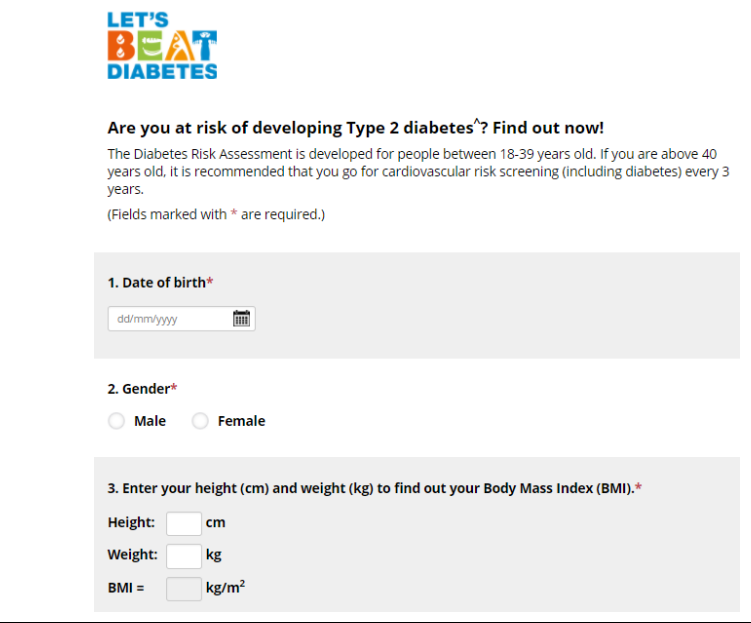
\includegraphics[width=0.5\paperwidth]{C:/Users/Admin/Desktop/Github/question_bank/LyX/static/img/9597-DHS-2017-P2-Q1-2}
\par\end{center}

\begin{center}
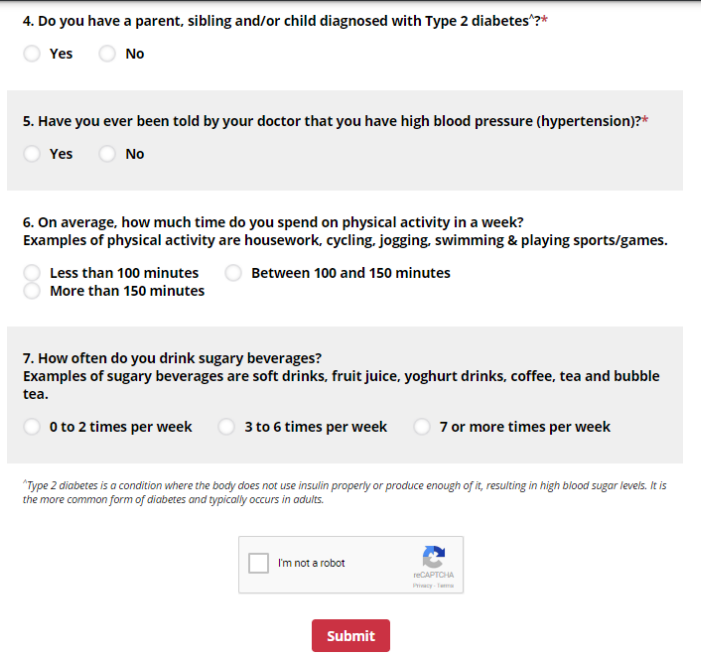
\includegraphics[width=0.5\paperwidth]{C:/Users/Admin/Desktop/Github/question_bank/LyX/static/img/9597-DHS-2017-P2-Q1-3}
\par\end{center}
\end{enumerate}
\item You are tasked to setup a wireless network to provide mobile access
to the Internet so that users can record and retrieve their real-time
fitness data on the go. 
\begin{enumerate}
\item Name and describe four major physical components that may be found
in a wireless network. \hfill{}{[}4{]}
\item What is the purpose of SSID?\hfill{} {[}1{]}
\end{enumerate}
\item Given the relationship: bit rate = baud rate {*} voltage (\# bits
per signal) 
\begin{enumerate}
\item Explain the difference between baud rate and bit rate.\hfill{} {[}2{]}
\item The following voltage levels expressed in volts are chosen to encode
bits: 

-6.0, -4.5, -3.0, -1.5, +1.5, +3.0, +4.5, +6.0 

How many bits represent these voltages? \hfill{}{[}1{]}
\item For the above voltages, write down one possible set of corresponding
bit patterns.\hfill{} {[}1{]}
\item If the baud rate of the line is 900 baud what is the bit rate for
the voltage levels? \hfill{}{[}1{]}
\end{enumerate}
\end{enumerate}
{[}SPLIT\_HERE{]}
\item \textbf{{[}DHS/PRELIM/9597/2017/P2/Q2{]} }

You are provided with an array S of non-negative floating point numbers
representing the daily starting stock prices of a company over a given
day range. 
\begin{enumerate}
\item Design a quadratic time complexity $O(n^{2})$ algorithm to determine
the maximum profit that could have been made by buying and then selling
the stock. Explain why your algorithm has this efficiency. \hfill{}{[}5{]}
\item Design a more efficient (either linearithmic $O(n\log n)$ or linear
$O(n)$) algorithm to determine the maximum profit. Explain why your
algorithm has this time complexity. \hfill{}{[}5{]}
\end{enumerate}
{[}SPLIT\_HERE{]}
\item \textbf{{[}DHS/PRELIM/9597/2017/P2/Q3{]} }

You are given 25 distinct integers and a function \texttt{Sort5} that
can sort 5 integers in one call.
\begin{enumerate}
\item Which sorting function would you use for \texttt{Sort5} and why?\hfill{}
{[}3{]}
\item Design an algorithm to determine the largest, second largest and third
largest integers amongst the 25 integers using the \texttt{Sort5}
function. Minimise the number of calls to \texttt{Sort5}.\hfill{}
{[}7{]}
\end{enumerate}
{[}SPLIT\_HERE{]}
\item \textbf{{[}DHS/PRELIM/9597/2017/P2/Q4{]} }

The following questions relate to a binary search tree (BST) whose
keys are the first 16 prime numbers: 2, 3, 5, 7, 11, 13, 17, 19, 23,
29, 31, 37, 41, 43, 47, 53. 
\begin{enumerate}
\item Draw the BST given its preorder traversal: 19, 7, 3, 2, 5, 11, 17,
13, 43, 23, 37, 29, 31, 41, 47, 53.\hfill{} {[}2{]}
\item Design an algorithm that takes as input a BST and a value, and returns
the first key \texttt{k} that would appear in an inorder traversal
which is greater than value. What is the efficiency of your algorithm?\hfill{}
{[}4{]}
\item Design a more efficient algorithm to determine \texttt{k}. What is
the efficiency of your improved algorithm? Explain why this algorithm
is more efficient.\hfill{} {[}4{]}
\end{enumerate}
{[}SPLIT\_HERE{]}
\item \textbf{{[}DHS/PRELIM/9597/2017/P2/Q5{]} }

A website hosting company keeps details of its members. Each member
has a unique id and name. The company offers two types of membership:
Free and Paid. Each free member is able to host a personal static
website, while each paid member can host a dynamic website with a
database for a monthly fee and is also provided with a helpdesk support
email. 

The business owner employs a developer to use object-oriented programming
to store and process its members' data. 
\begin{enumerate}
\item Draw a class diagram showing the relationship between the different
memberships. \hfill{}{[}4{]}
\item Using appropriate examples, explain the following terms: 
\begin{enumerate}
\item encapsulation 
\item inheritance 
\item polymorphism\hfill{} {[}6{]}
\end{enumerate}
\item The business owner intends to reorganise the membership model. The
paid membership will be changed to a Monthly one and a new Annual
membership will be introduced. An annual member will pay its fee annually
with a 2-month discount, and have access to a dedicated helpdesk support
hotline. Explain how this reorganisation will affect your design in
\textbf{part (a)}.\hfill{} {[}5{]}
\end{enumerate}
{[}SPLIT\_HERE{]}
\item \textbf{{[}DHS/PRELIM/9597/2017/P2/Q6{]} }

The following figure shows the entry proof of a student for the Singapore-Cambridge
GCE A-Level Examination. 

\noindent\fbox{\begin{minipage}[t]{1\columnwidth - 2\fboxsep - 2\fboxrule}%
2017 SINGAPORE-CAMBRIDGE GCE A-LEVEL EXAMINATION 

Entry Proof for School Candidates 

Statutory Name : LIM AH SENG 

NRIC : S9987654A 

Centre / Index No. : 3042 / 1234

Academic Level : JC 2 

School Name : RESERVED JUNIOR COLLEGE 

Class Name : 23

\begin{tabular}{|c|c|c|c|c|c|c|}
\hline 
Subject Code / Paper & Subject Name & Mode of Assessment & School Code & Exam Date & Start Time & Duration\tabularnewline
\hline 
9749 / 04 & H2 PHYSICS & SCIENCE PRACTICAL  &  & 16-OCT-2017 &  & 2 hr 30 min\tabularnewline
\hline 
8807 / 01 & H1 GENERAL PAPER & WRITTEN & 3101 & 06-NOV-2017 & 08:00 & 1 hr 30 min\tabularnewline
\hline 
8807 / 02 & H1 GENERAL PAPER & WRITTEN & 3101 & 06-NOV-2017 & 10:30 & 1 hr 30 min\tabularnewline
\hline 
8872 / 02 & H1 CHEMISTRY & WRITTEN & 3101 & 07-NOV-2017 & 08:00 & 2 hr 0 min\tabularnewline
\hline 
9758 / 01 & H2 MATHEMATICS & WRITTEN & 3101 & 09-NOV-2017 & 08:00 & 3 hr 0 min\tabularnewline
\hline 
9758 / 02 & H2 MATHEMATICS & WRITTEN & 3101 & 13-NOV-2017 & 08:00 & 3 hr 0 min\tabularnewline
\hline 
9749 / 02 & H2 PHYSICS & WRITTEN & 3101 & 16-NOV-2017 & 08:00 & 2 hr 0 min\tabularnewline
\hline 
9749 / 03 & H2 PHYSICS  & WRITTEN & 3101 & 22-NOV-2017 & 14:00 & 2 hr 0 min\tabularnewline
\hline 
9753 / 01  & H2 MUSIC & WRITTEN & 3101 & 27-NOV-2017 & 14:00 & 2 hr 30 min\tabularnewline
\hline 
8872 / 01 & H1 CHEMISTRY & WRITTEN & 3101 & 29-NOV-2017 & 14:00 & 0 hr 50 min\tabularnewline
\hline 
9749 / 01 & H2 PHYSICS & WRITTEN & 3101 & 01-DEC-2017 & 14:30 & 1 hr 0 min\tabularnewline
\hline 
9753 / 21 & H2 MUSIC & PRACTICAL &  &  &  & 0 hr 25 min\tabularnewline
\hline 
9753 / 32 & H2 MUSIC & COURSEWORK & 3101 &  &  & \tabularnewline
\hline 
9819 / 01 & H3 MUSIC & PROJECT-BASED & 3101 &  &  & \tabularnewline
\hline 
\textbf{School Code} & \multicolumn{2}{c|}{Centre Name} & \multicolumn{4}{c|}{\textbf{Address}}\tabularnewline
\hline 
3101 & \multicolumn{2}{c|}{RESERVED JUNIOR COLLEGE} & \multicolumn{4}{c|}{12 WALKOVER STREET. SINGAPORE 345678}\tabularnewline
\hline 
\end{tabular}%
\end{minipage}}

The exam board wishes to manage this information using a relational
database. The normalised design requires a number of tables. 
\begin{enumerate}
\item Draw an Entitiy-Relationship (E-R) diagram that shows these tables
and the relationships between them.\hfill{} {[}4{]}
\item A table description can be expressed as:
\noindent \begin{center}
\texttt{TableName(}\texttt{\uline{Attribute1}}\texttt{, Attribute2,
Attribute3, \dots ) }
\par\end{center}

The primary key is indicated by underlining one or more attributes. 

Derive the table descriptions for the tables.\hfill{} {[}6{]}
\item There are some fields with missing or null values. Explain how these
arise and how a Database Management System (DBMS) may provide facilities
to ensure the information is appropriately managed.\hfill{} {[}3{]}
\item The DBMS also contains a report generation facility for producing
formatted output. Name one component used in the report generator
and how it is related to data stored in the tables.\hfill{} {[}2{]}
\end{enumerate}
{[}SPLIT\_HERE{]}
\end{enumerate}

\end{document}
